\documentclass{article}
\usepackage{graphicx}
\usepackage{amsmath}
\usepackage{amsfonts}
\usepackage{rotating}

\renewcommand{\labelenumii}{\theenumii}
\renewcommand{\theenumii}{\theenumi.\arabic{enumii}.}

\title{NEW Energy plane\\ Status report May 2016}

\author{V.~\'Alvarez, S.~C\'arcel, A.~Laing,
  I.~Liubarsky, A.~Mart\'inez, J. Rodriguez, V. Herrero \\ and J.J. G\'omez-Cadenas}

\begin{document}

\maketitle

\begin{abstract}
  This document contains a description of the work performed and
  ongoing related to the realisation of the safe and efficient installation of all components related to the energy plane of NEW.
\end{abstract}

\newpage

\tableofcontents

\newpage

\section{Energy plane design}
\label{sec:design}
The energy plane (shown in figure~\ref{fig:des})
consists of a 11 ~cm thick copper support plate with 12 copper window
covered with brazed sapphire windows fixed to the front of the plate. The
set-up as a whole seals the pressure vessel from the PMT-region,
which is held at vacuum levels of
$<10^{-4}$~mbar. Additional copper shielding fixed to the
vacuum side of the apertures, offer further shielding against gammas traversing the PMTs and
entering in the detector volume. The 12 Hamamatsu R11410 PMTs are optically coupled to 
the sapphire window using NyoGel OCK-451. The sensors are held in place by a plastic brace and spring.

\begin{figure}[tph!]
  \begin{center}
    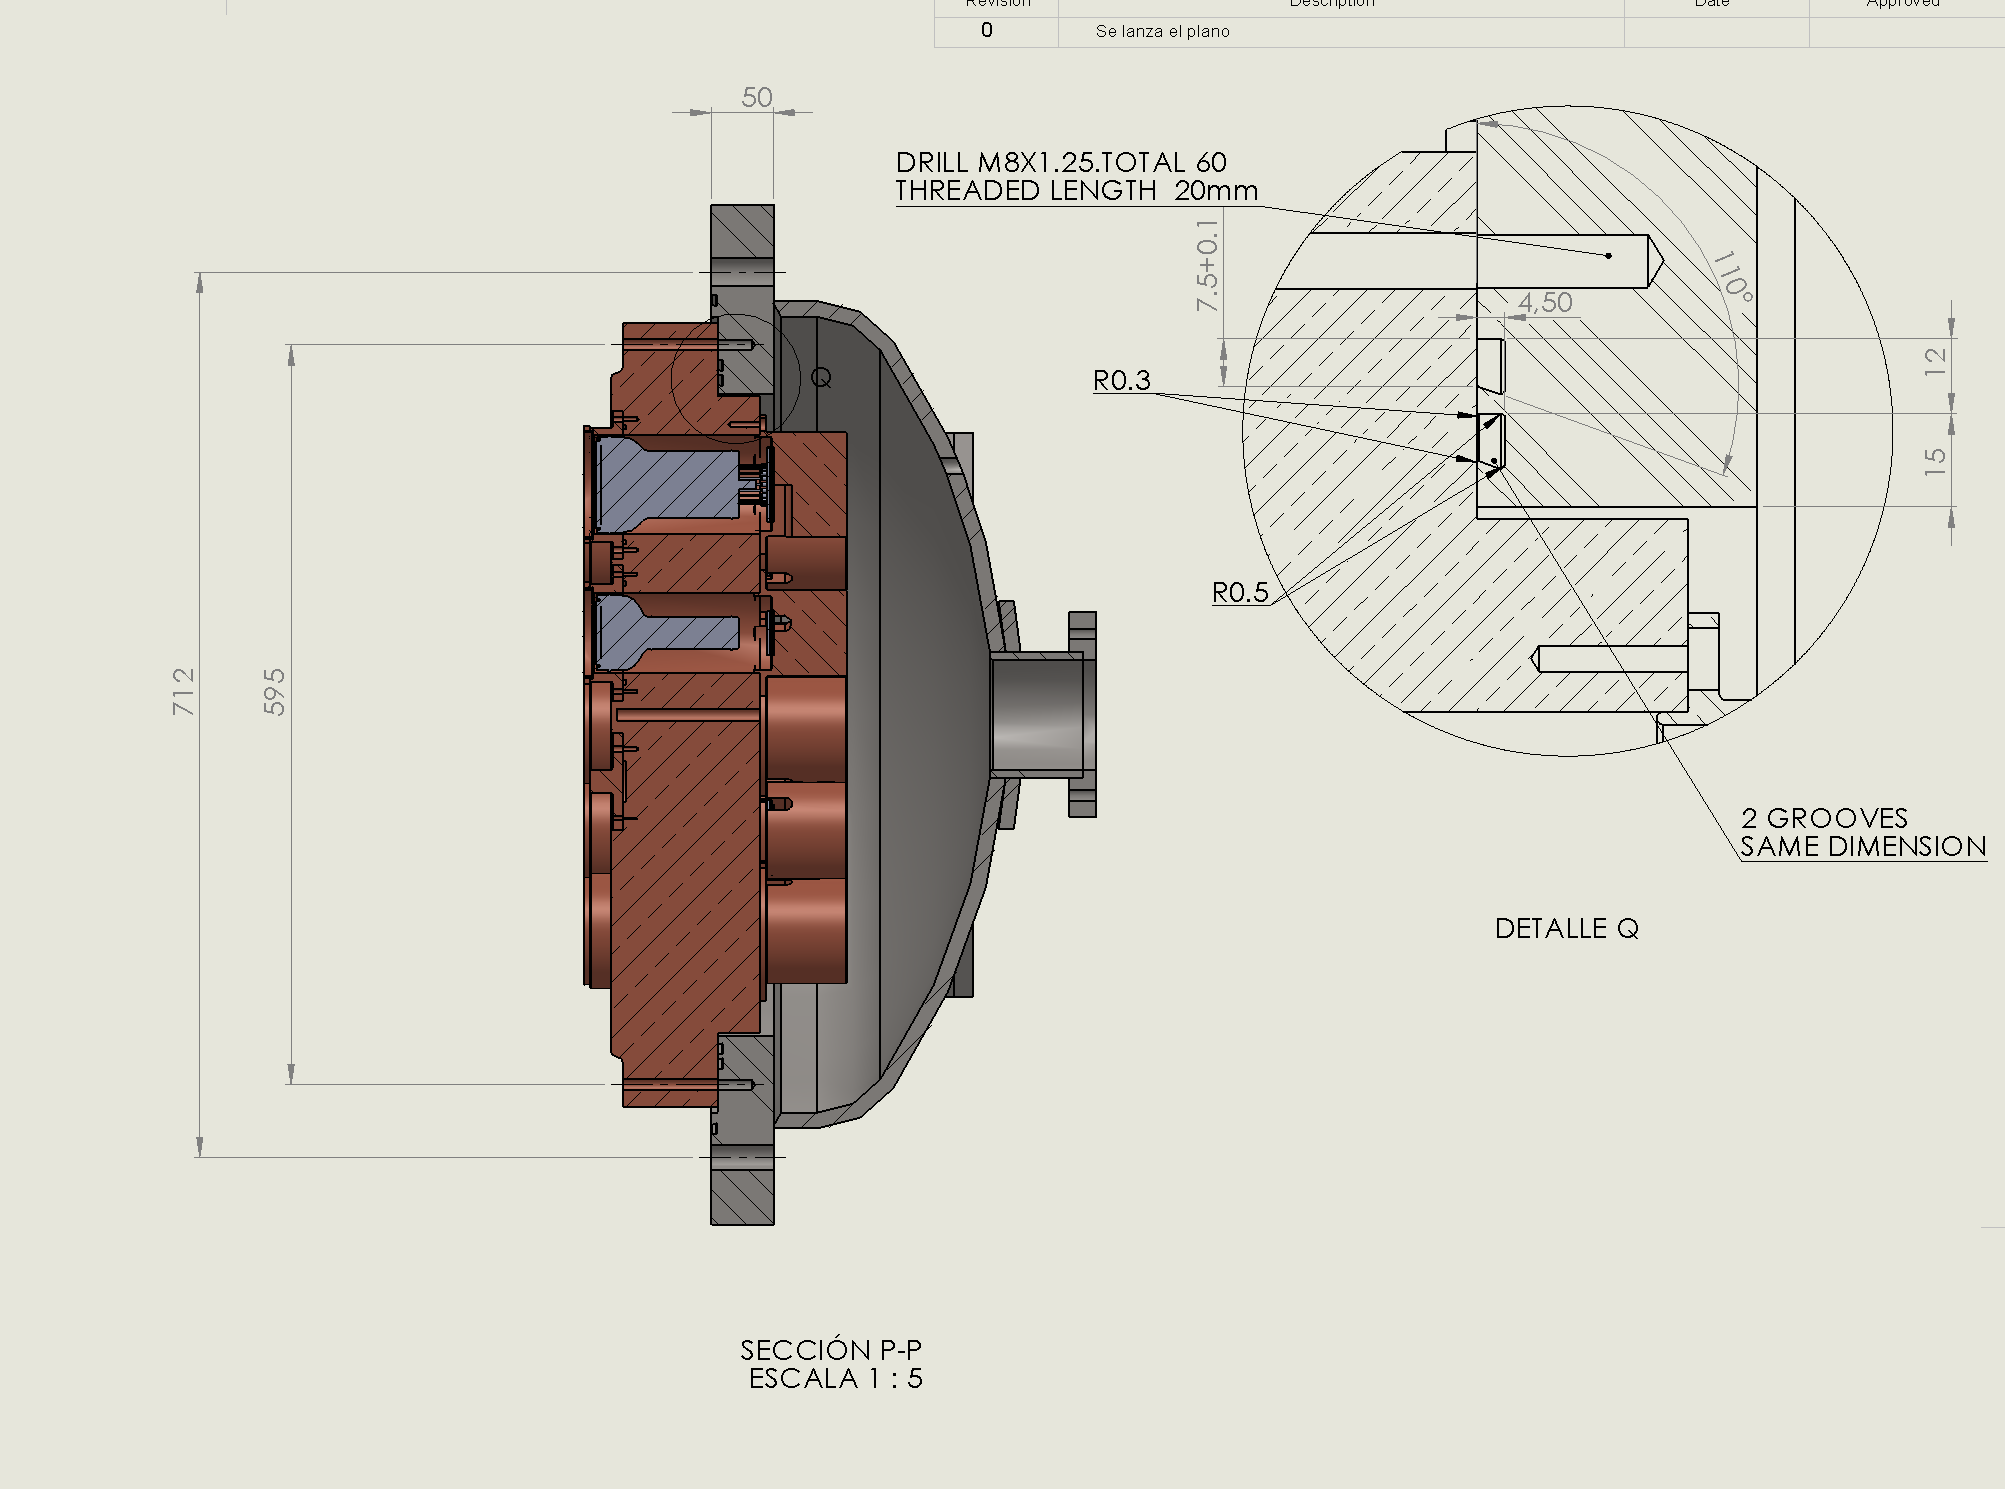
\includegraphics[height=4cm,width=0.45\textwidth]{img/SUPERCAN}
%    \includegraphics[height=4cm,width=0.45\textwidth]{img/SUPERCAN_1} \\
    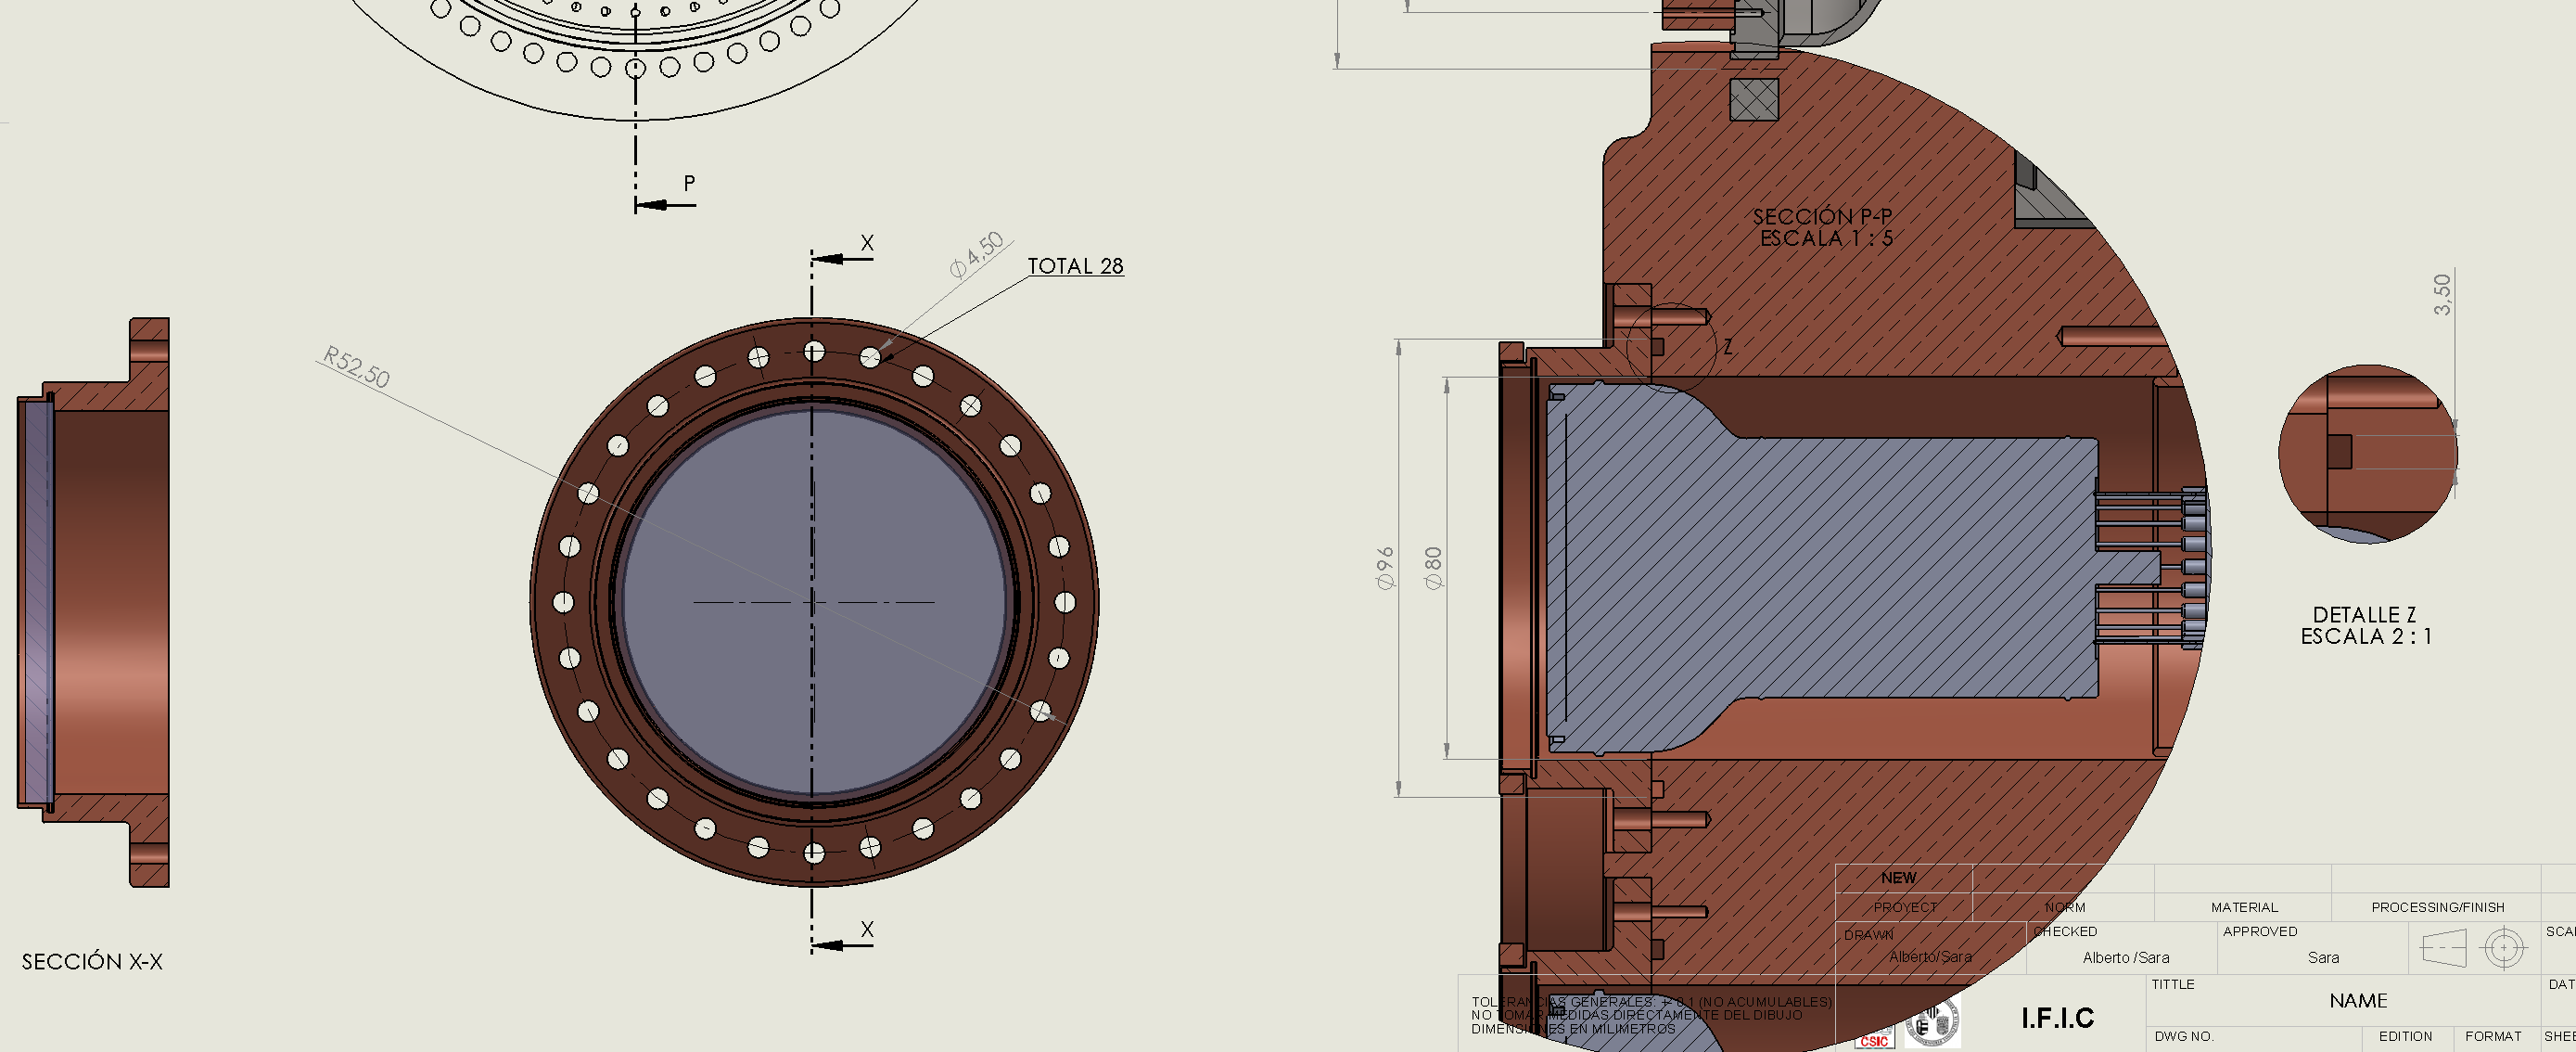
\includegraphics[height=4cm,width=0.45\textwidth]{img/SUPERCAN_3}
	  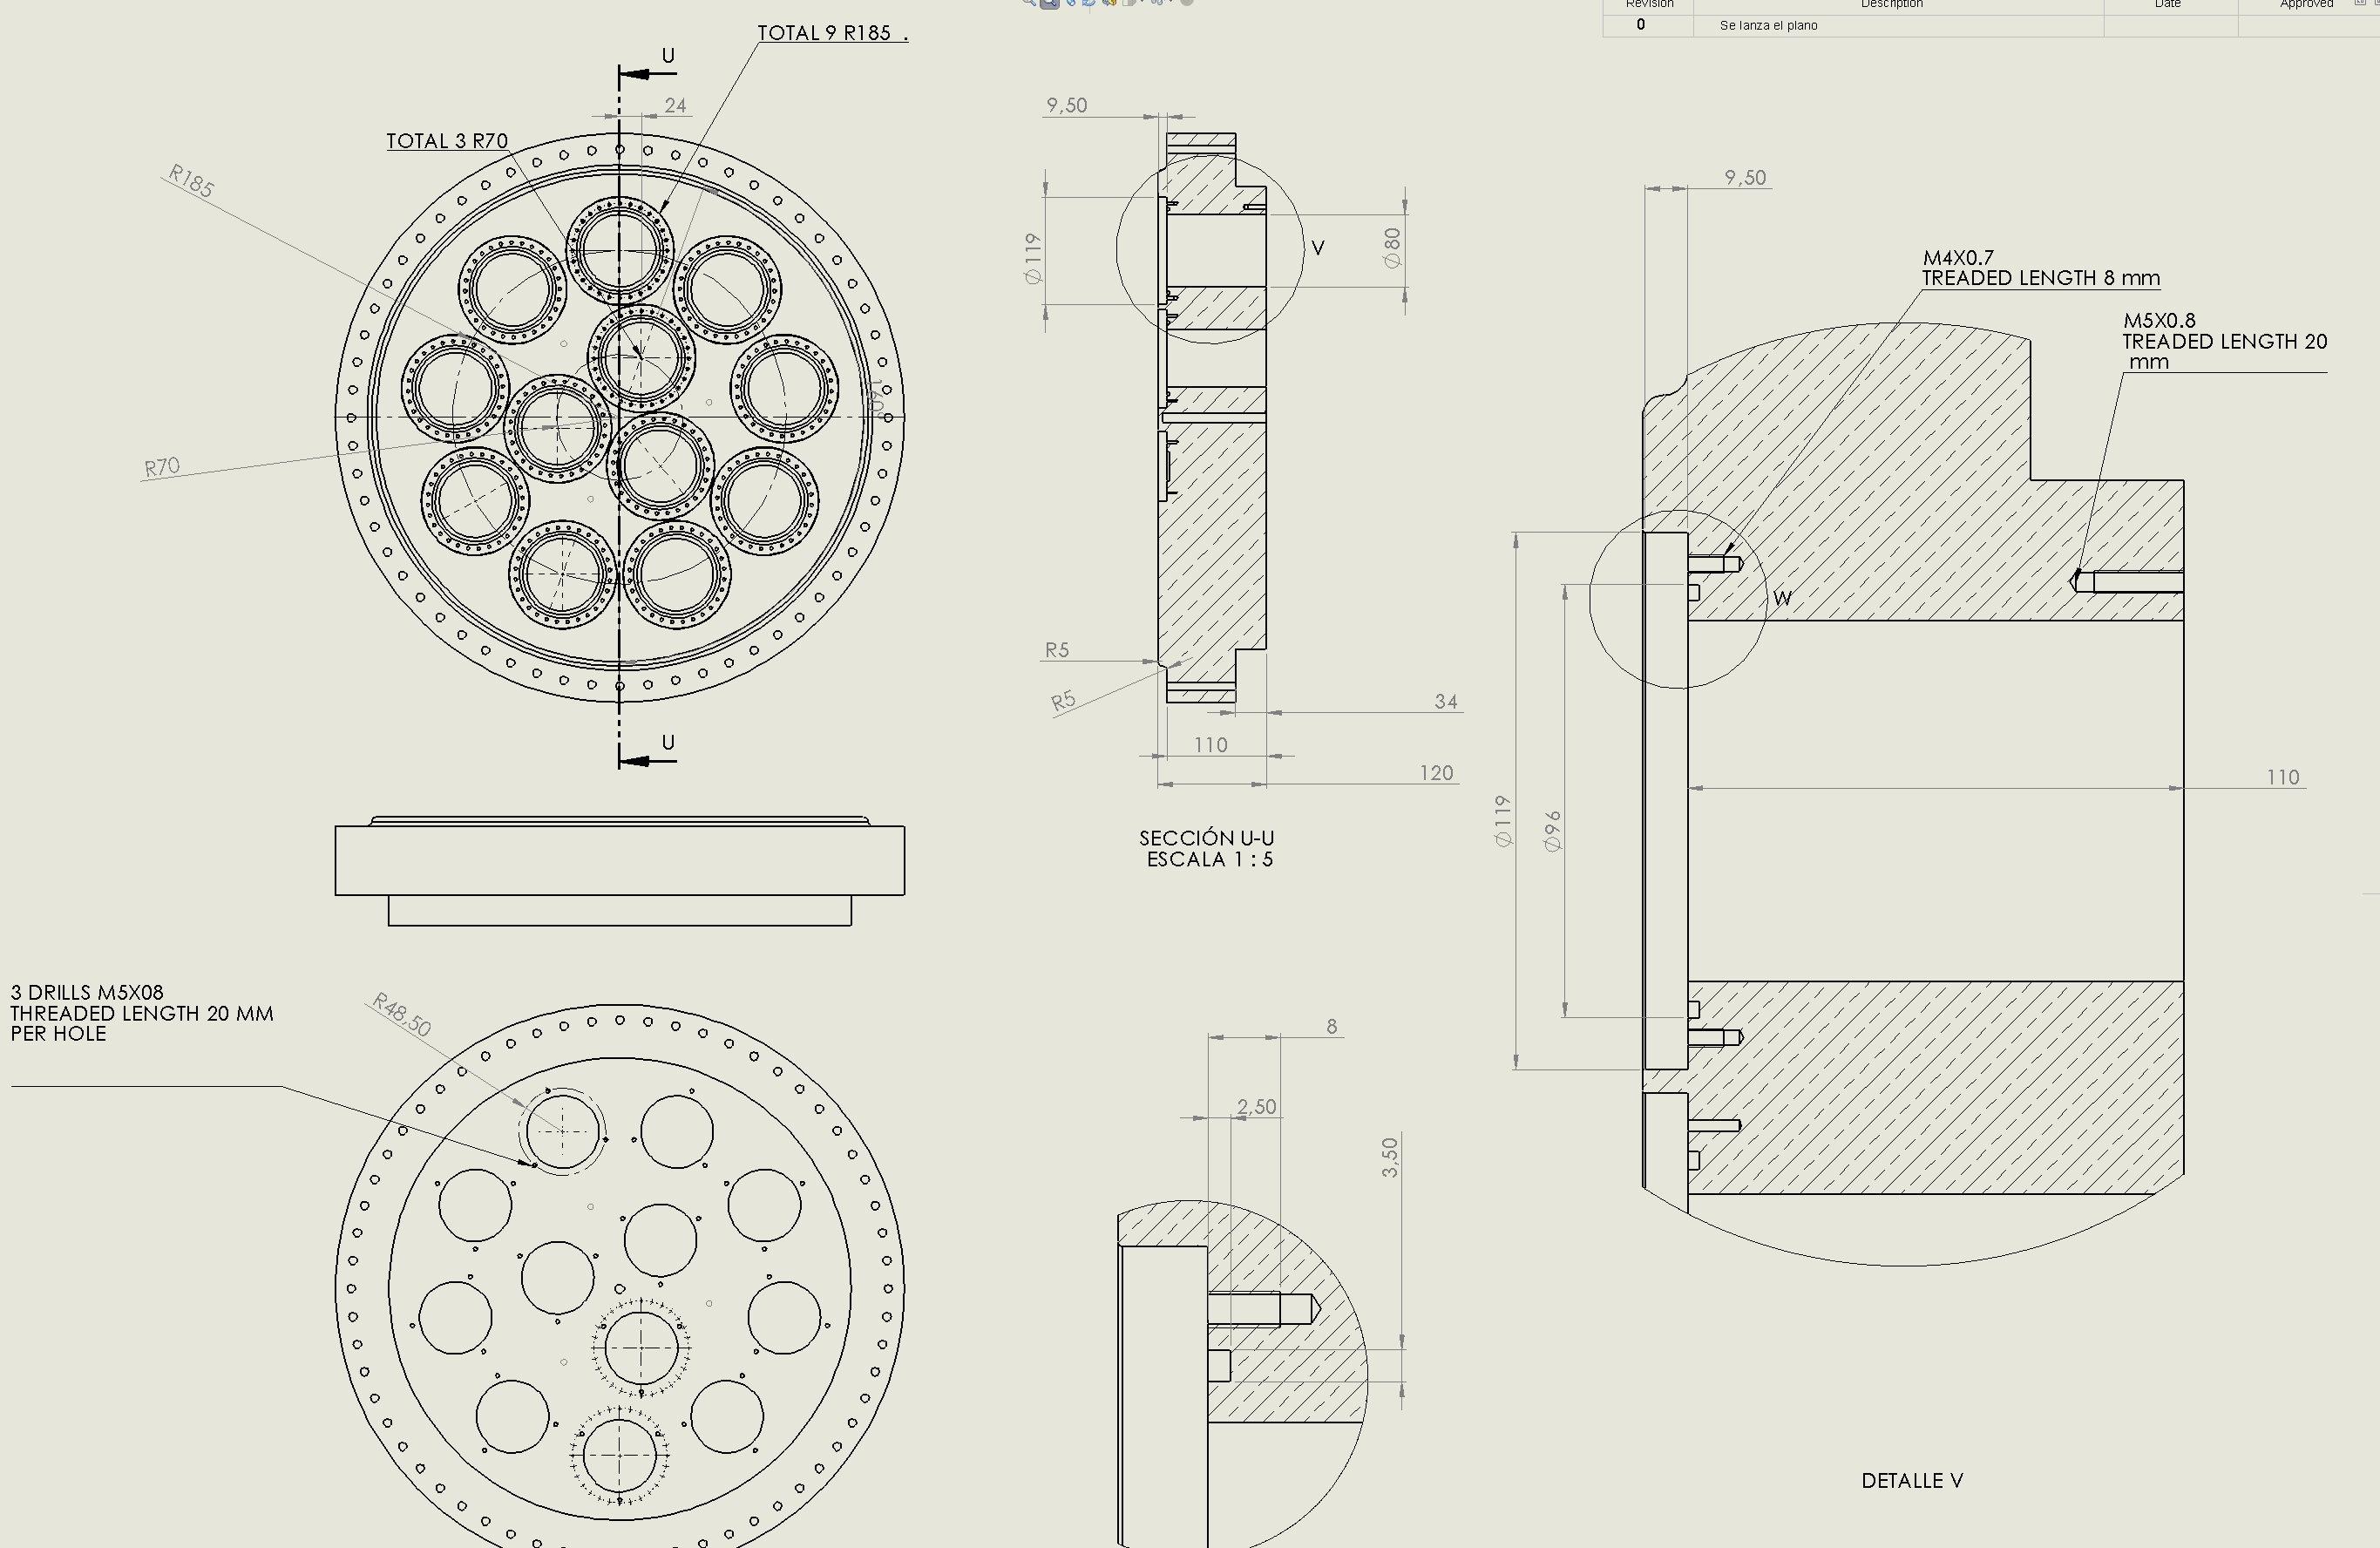
\includegraphics[height=4cm,width=0.45\textwidth]{img/SUPERCAN_2}
  \end{center}
  \caption{Tecnical drawings for the energy plane. }
  \label{fig:des}
\end{figure}

The PMTs receive high voltage and have their signal extracted via a
shielded twisted pair cable connected to a feedthrough in the energy-plane head. The distribution of
signal and supply at each individual PMT is controlled via a
Kapton circuit board (base), covered with a
copper cap filled with epoxy and connected to the support plate. The cap acts as a heat sink.

Figure \ref{fig:des} shows a transversal cut of the design of the energy plane and a frontal view of the copper mother-can. The PMTs position is clearly visible in the frontal view. 

\section{Progress in preparation for installation}
\label{sec:EPProg}

The energy plane has been installed in the NEW apparatus. Figure \ref{fig:energy_installation} shows different stages of the installation process. The most relevant steps were:
\begin{itemize}
\item The copper support plate (mother-can) has been installed in NEW vessel.
\item 14 sapphire windows have been successfully brazed to their copper window frames. 12 windows are properly installed in the mother can.
\item 14 sapphire windows have been coated with PEDOT using spin coating technique at the ICMol facilities.
\item 14 sapphire windows have been coated with TPB.
\item PMTs have been cabled up to the DAQ.
\item The PMT bases have been potted into their copper heat sinks using epoxy.
\item The PMT bases have been tested inside the detector.
\end{itemize}


\begin{figure}
  \begin{center}
    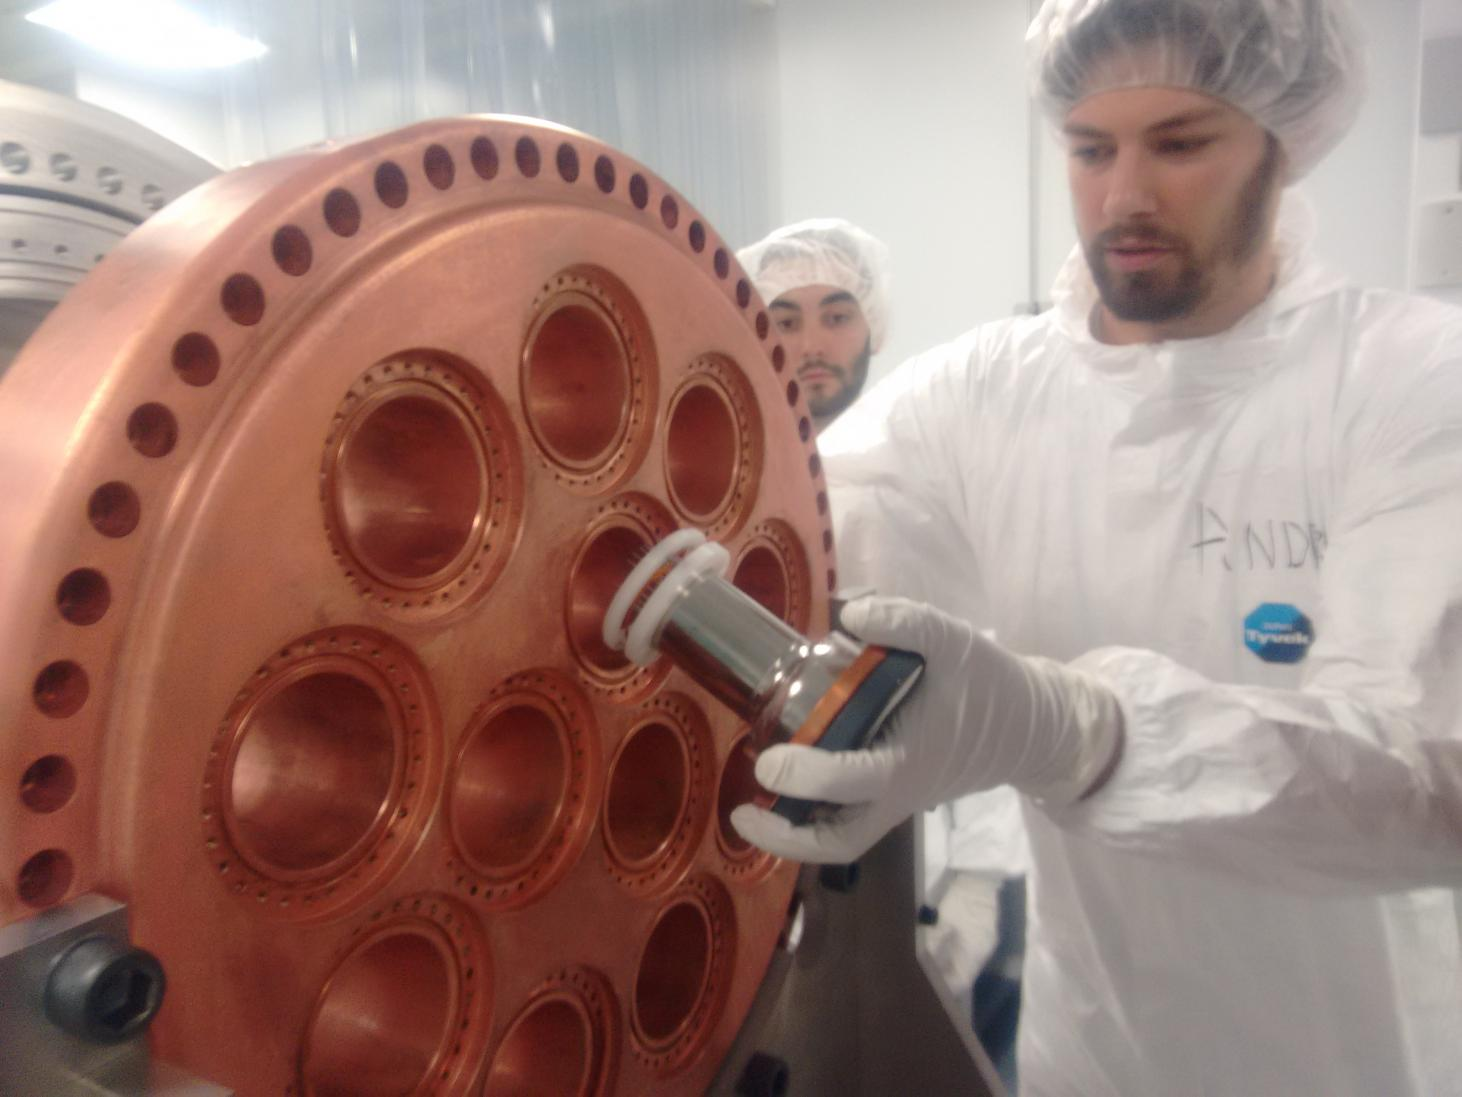
\includegraphics[height=4cm,width=0.45\textwidth]{img/Andrew_pmt.jpg}
	  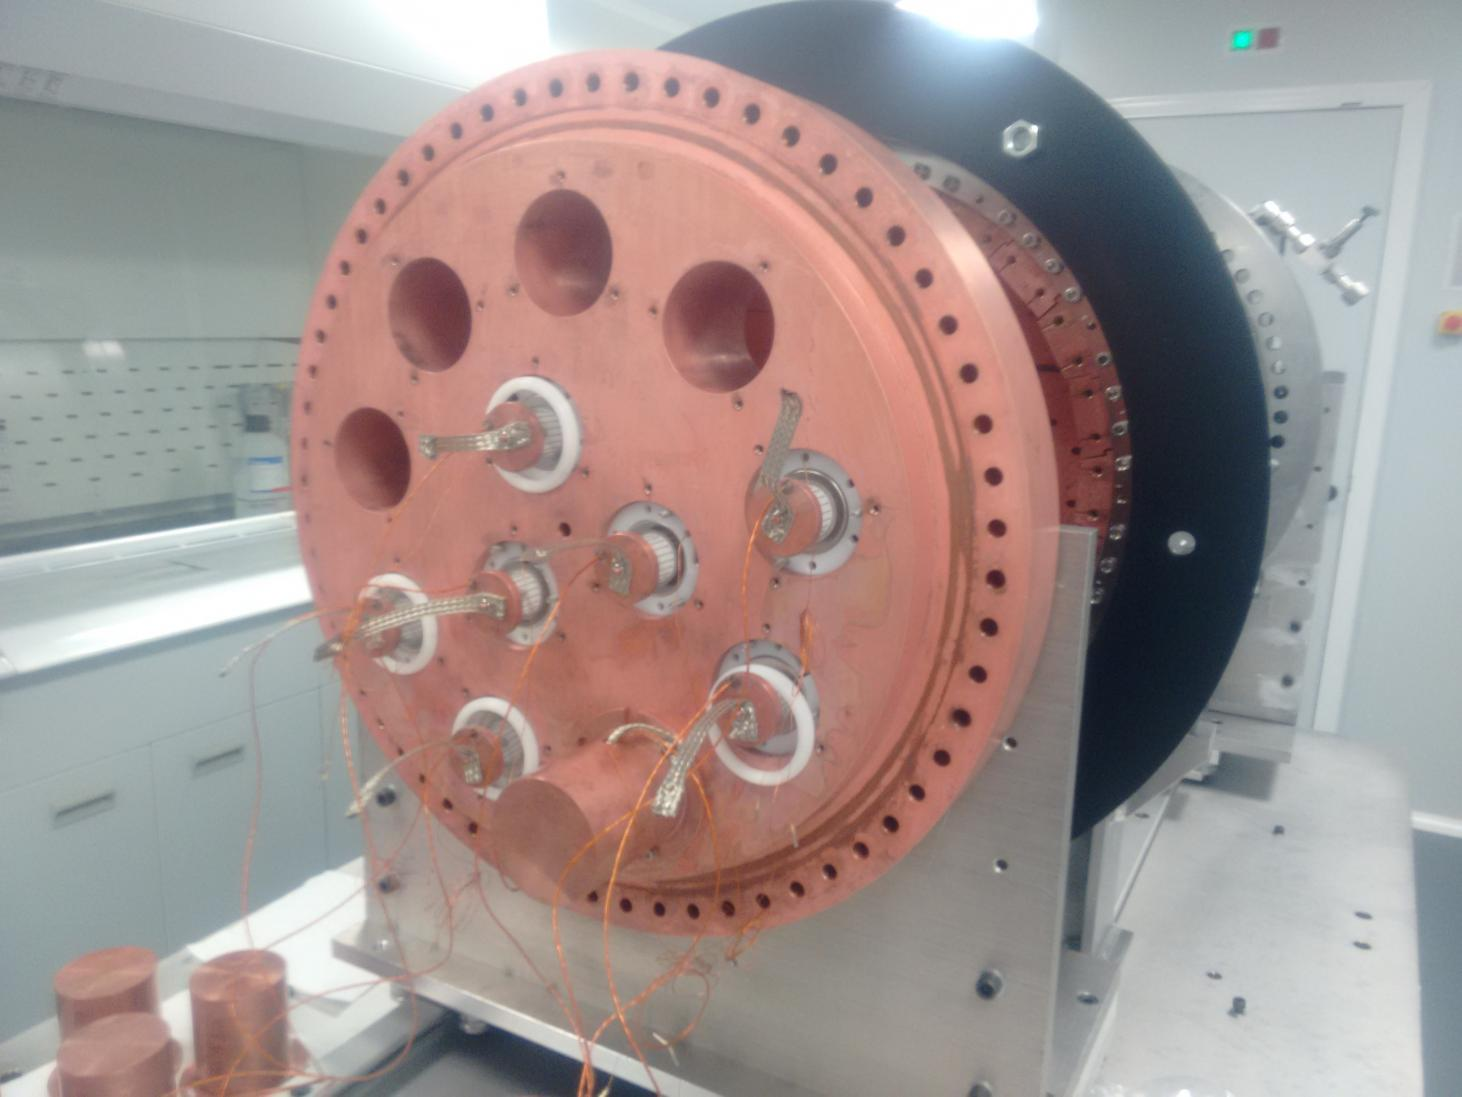
\includegraphics[height=4cm,width=0.45\textwidth]{img/PMTsback}
    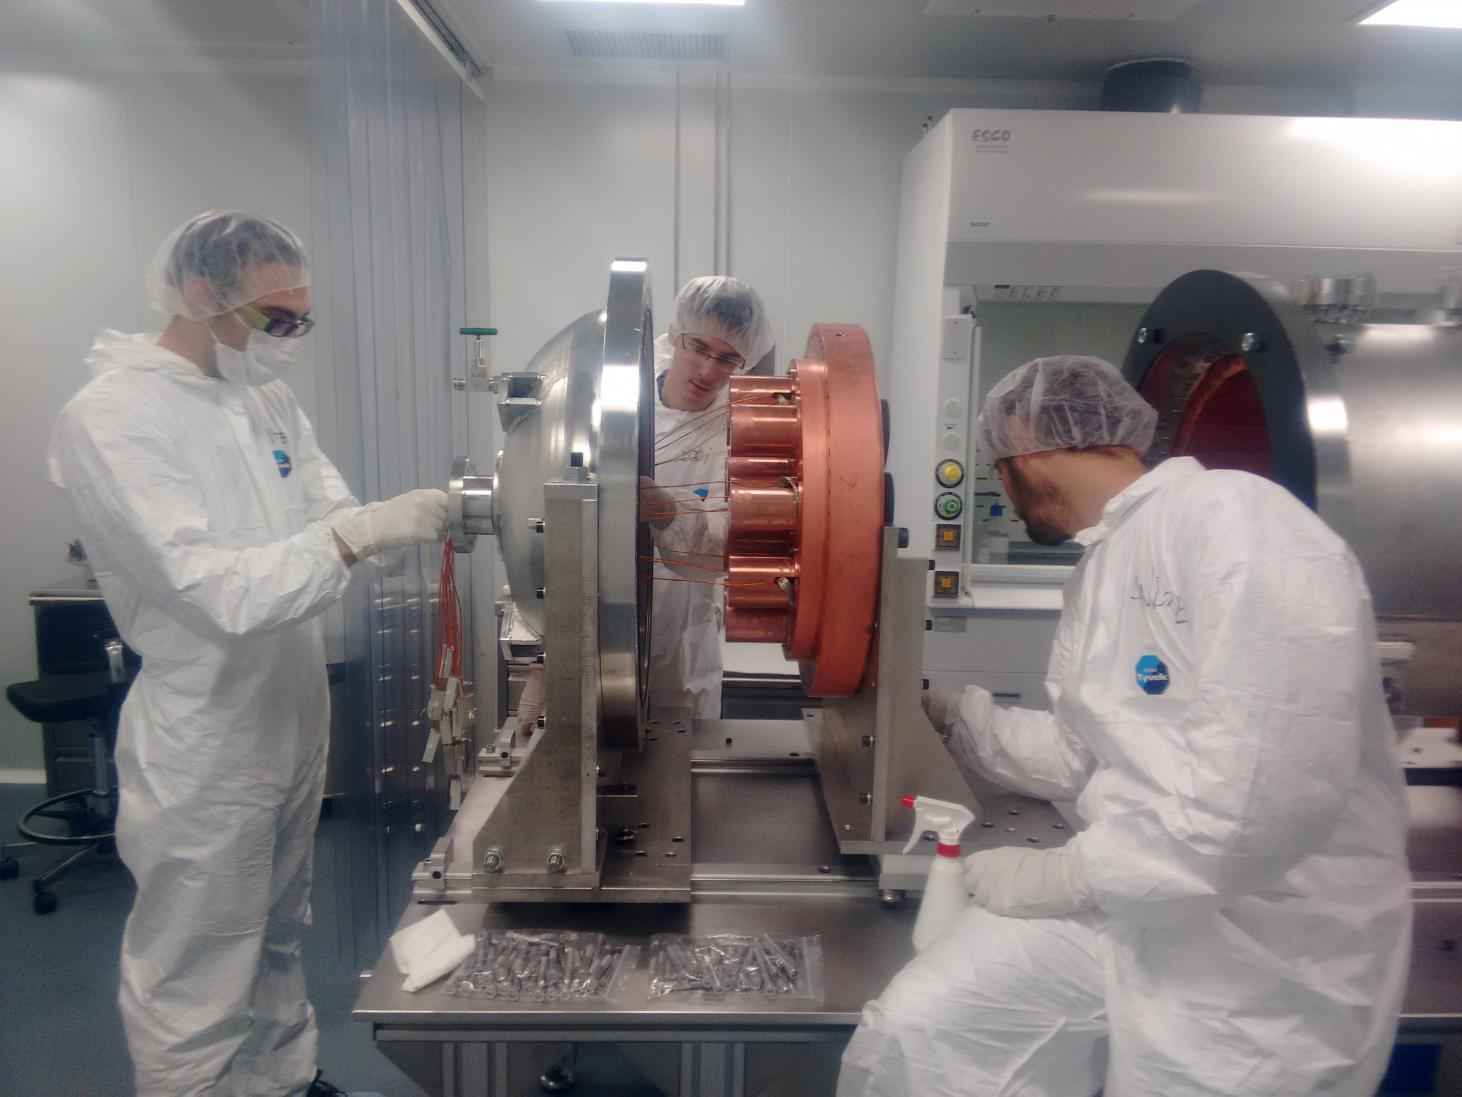
\includegraphics[height=4cm,width=0.45\textwidth]{img/cabling}
	 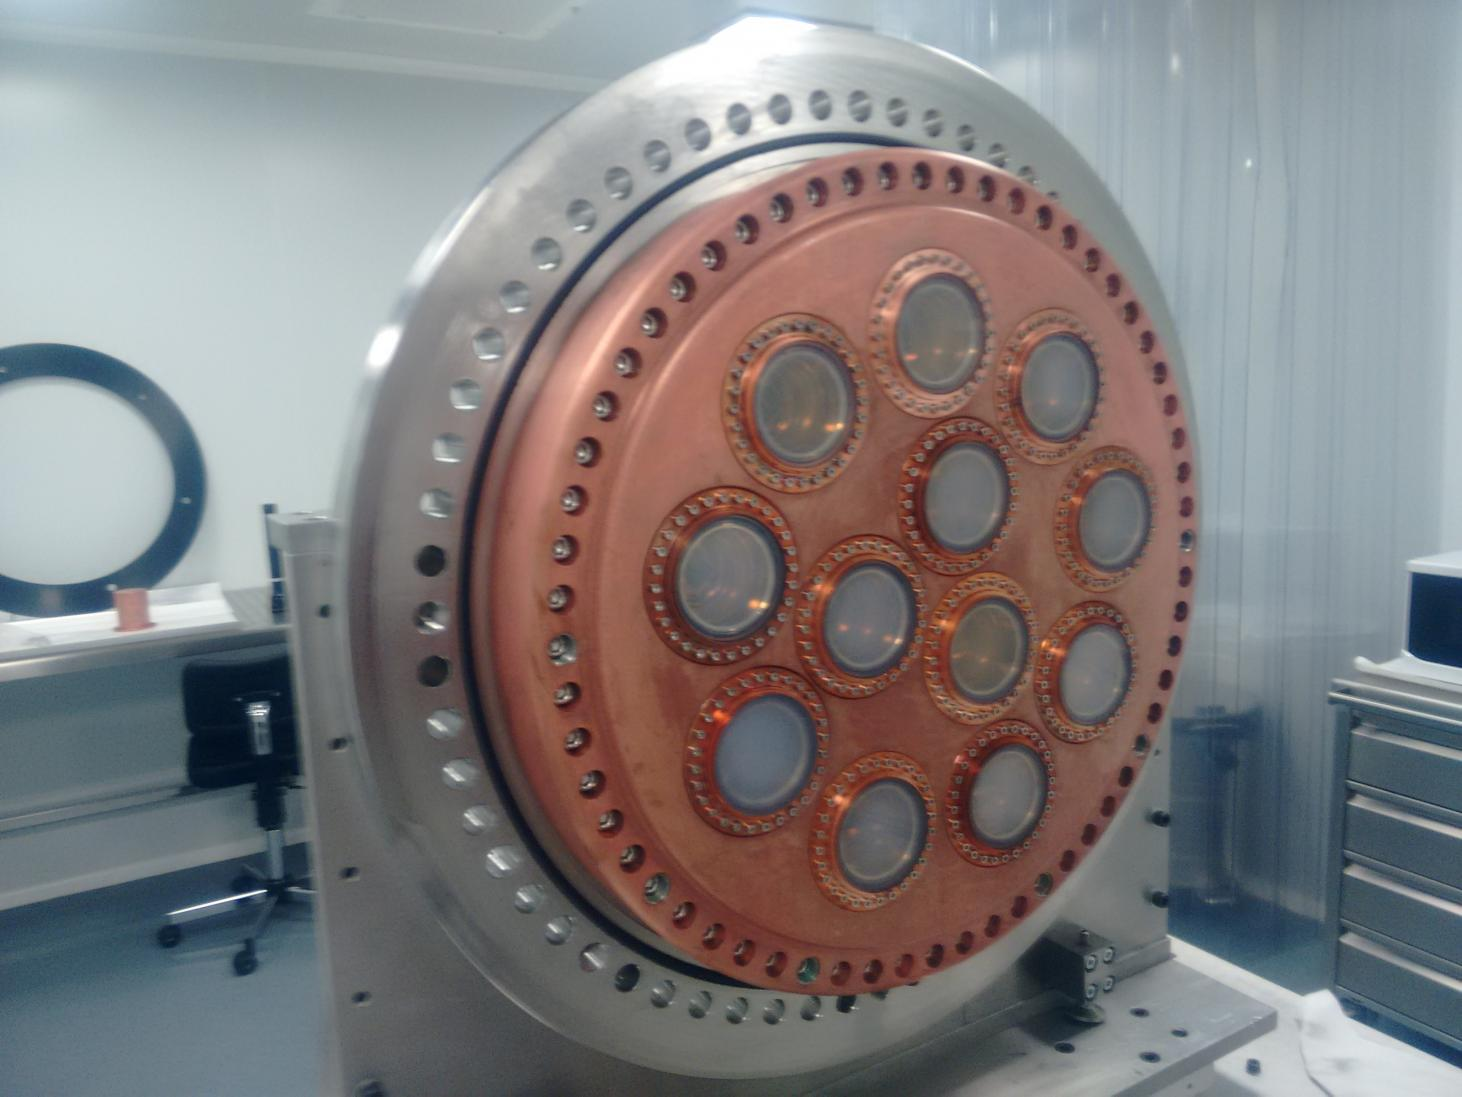
\includegraphics[height=4cm,width=0.45\textwidth]{img/full_energyplane} \\
	  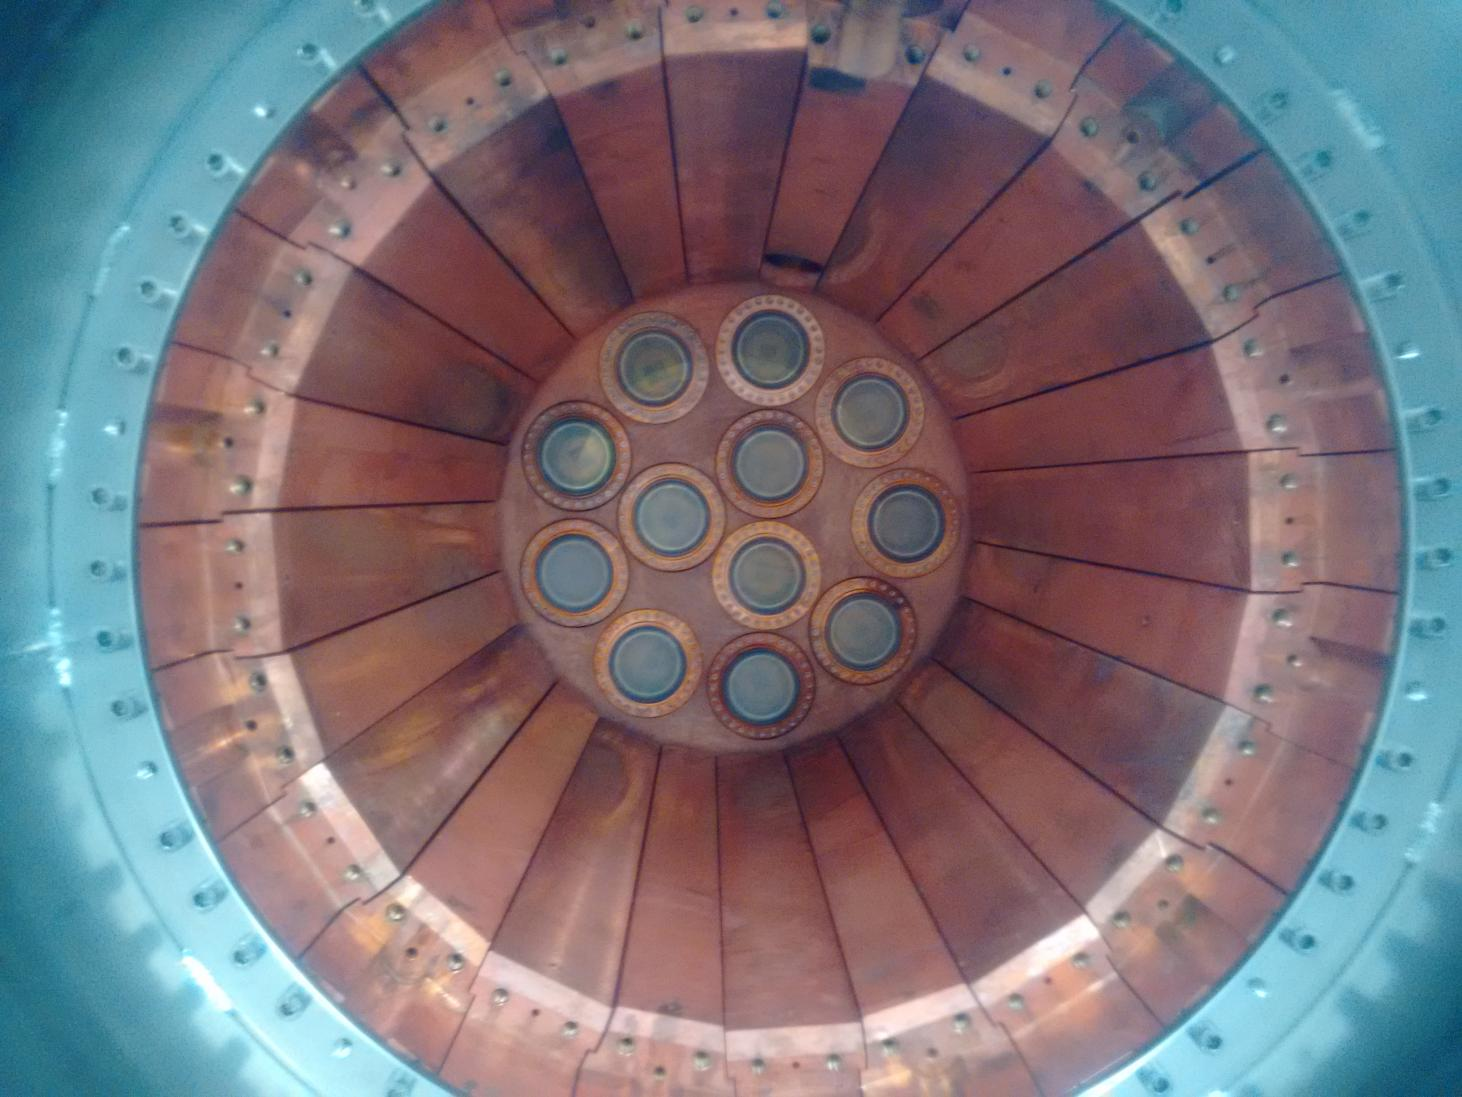
\includegraphics[height=4cm,width=0.45\textwidth]{img/full_energyplane_closed}
  \end{center}
  \caption{Different stages of the installation of the energy plane: Top left picture shows the positioning of the PMTs inside the mother can. Top right shows the back side of the mother can before the copper shielding for the PMTs is added. The copper hat covering the PMTs bases with the thermal contact cable is visible. Middle left shows the process of cabling and labelling the different PMTs. Middle right shows the energy plane once installed. The last picture, bottom, shows energy plane once the end-cap is closed.}
  \label{fig:energy_installation}
\end{figure}

\section{Energy Plane electronics}\label{sec:energy_fee}
After the firsts test with the PMTs and the whole electronic chain at LSC, two important issues were identified in the first design of the electronic chain: 
\begin{itemize}
\item The impedance of the high voltage differential cable was not well matched with the entering impedance of the de-coupling board of the FEE.
\item The decoupling capacitor was producing a negative overshoot in the signal that resulted in undesirable bipolar signals. 
\end{itemize}

These problems were not present in NEXT-DEMO since:
\begin{itemize}
\item Cable length was in the order of 1 m, so transmission line effects were not evident, unlike in the 10 m cable used for NEW.
\item Decoupling capacitors were not required, as a grounded-anode configuration was used. In NEW, a grounded-cathode scheme was chosen, so that the PMT bodies could at ground, in order to avoid problems with electrical insulation. 
\end{itemize}

To solve the above two issues, a full re-design of the bases and the FEE of the energy plane has taken place over the last two months. 
The new base design includes some of the components that were in the decoupling board previously. Other changes in the base are:

\begin{itemize}
\item The resistor chain has been slightly modified following the manufacturer (Hamamatsu) recommendations. 
\item Series resistors in the anode and in the last dynode have been added with the aim to damp reflections in the signal.
\item Capacitance values between dynodes have been modified to reduce the gain compression in the PMT for large signals.
\end{itemize}

Figure \ref{fig:fee_scheme} shows the new design for the front-end circuit. The main modifications to the previous design are:

\begin{itemize}
\item Differential and common-mode mode terminations have been added to the first stage's input. This has forced to change the first stage's topology.
\item In order to recover the signal's DC level and thus avoid bipolar pulses, an active integrator has been implemented in the second stage of the FEE.
\end{itemize}

The current circuit mitigates most of the problems but adds a new one: the integrator introduces a low-frequency (up to 10 kHz) walk in the signal's baseline.

The effect on the low-amplitude narrow S1 signal used for trigger can be minimized with a moving-average filter in the FPGA in the DAQ modules, 
which dynamically computes the baseline for each channel and subtracts it from the signal. At the time of writing this report, tests with actual PMT signals produce good results.

The effect on the larger-amplitude, wide (up to 100 microseconds) S2 signal used to measure energy is potentially more severe, as the baseline correction cannot be performed.
Aceptable signal-to-noise ratios (S/N) are expected with a number of enhancements which are currently being implemented. 
As an example, a factor of three in the S/N will be achieved just by replacing the current de-coupling capacitors with larger 8 nF ones. 

In the first half of May 2016, the new front-end circuit will be installed and tested in the NEW detector readout.

\begin{figure}
  \begin{center}
    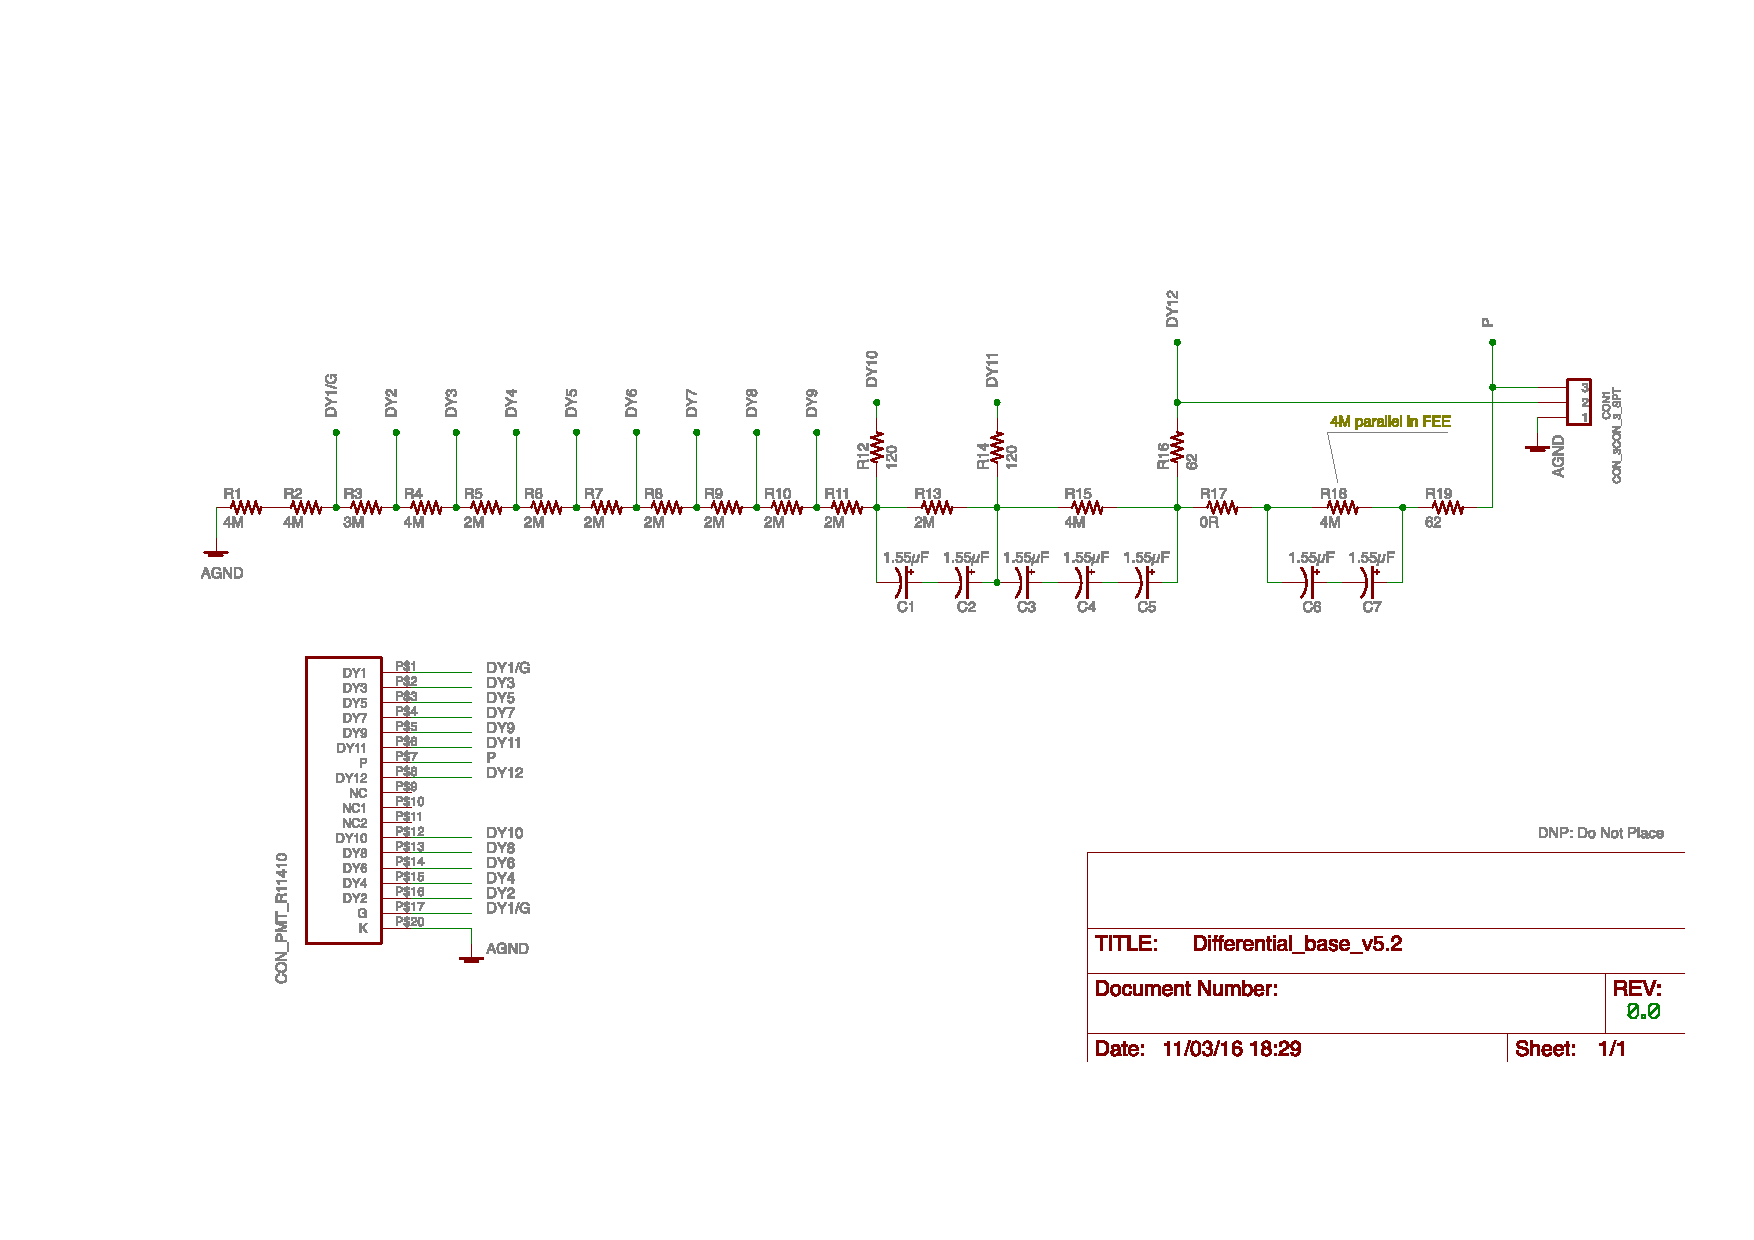
\includegraphics[height=4cm,width=0.95\textwidth]{img/Differential_base}
    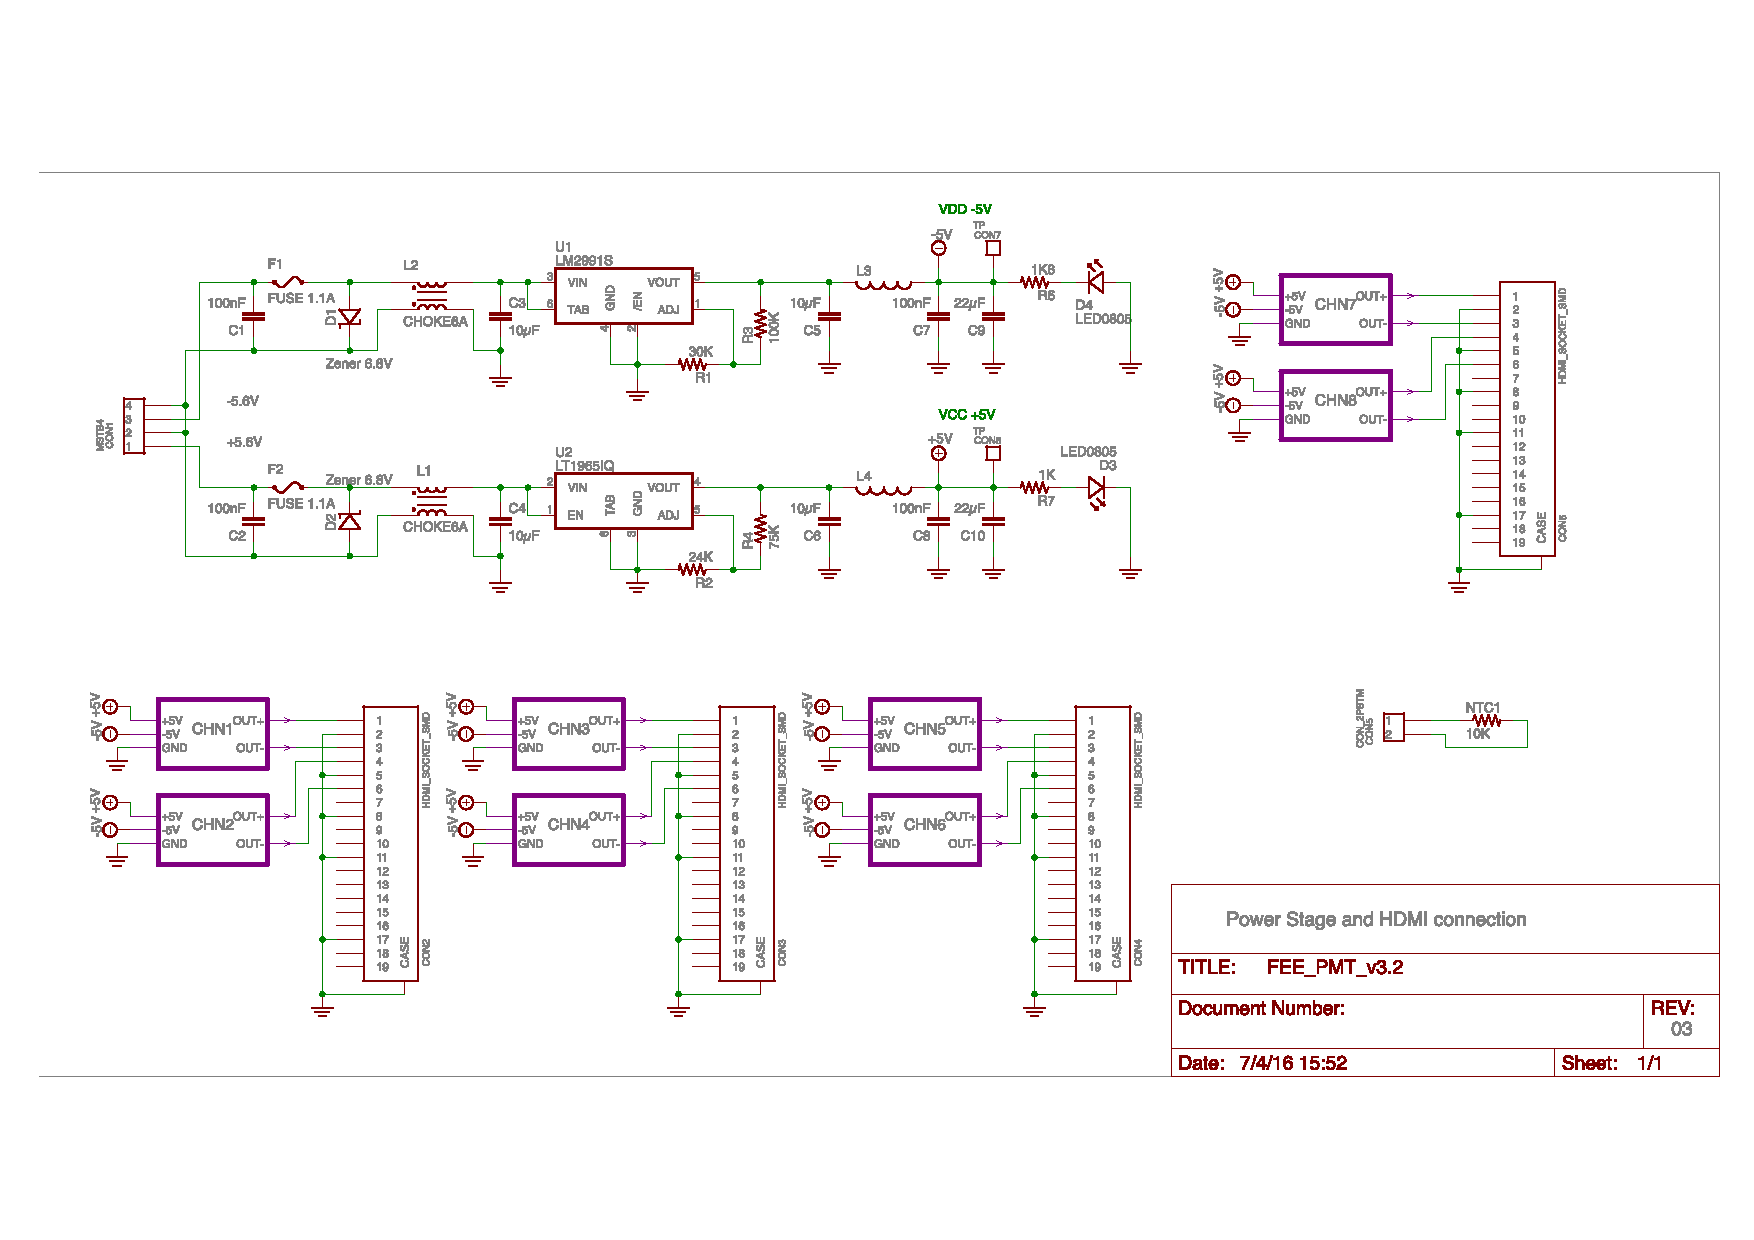
\includegraphics[height=4cm,width=0.95\textwidth]{img/de-coupling_board}
	  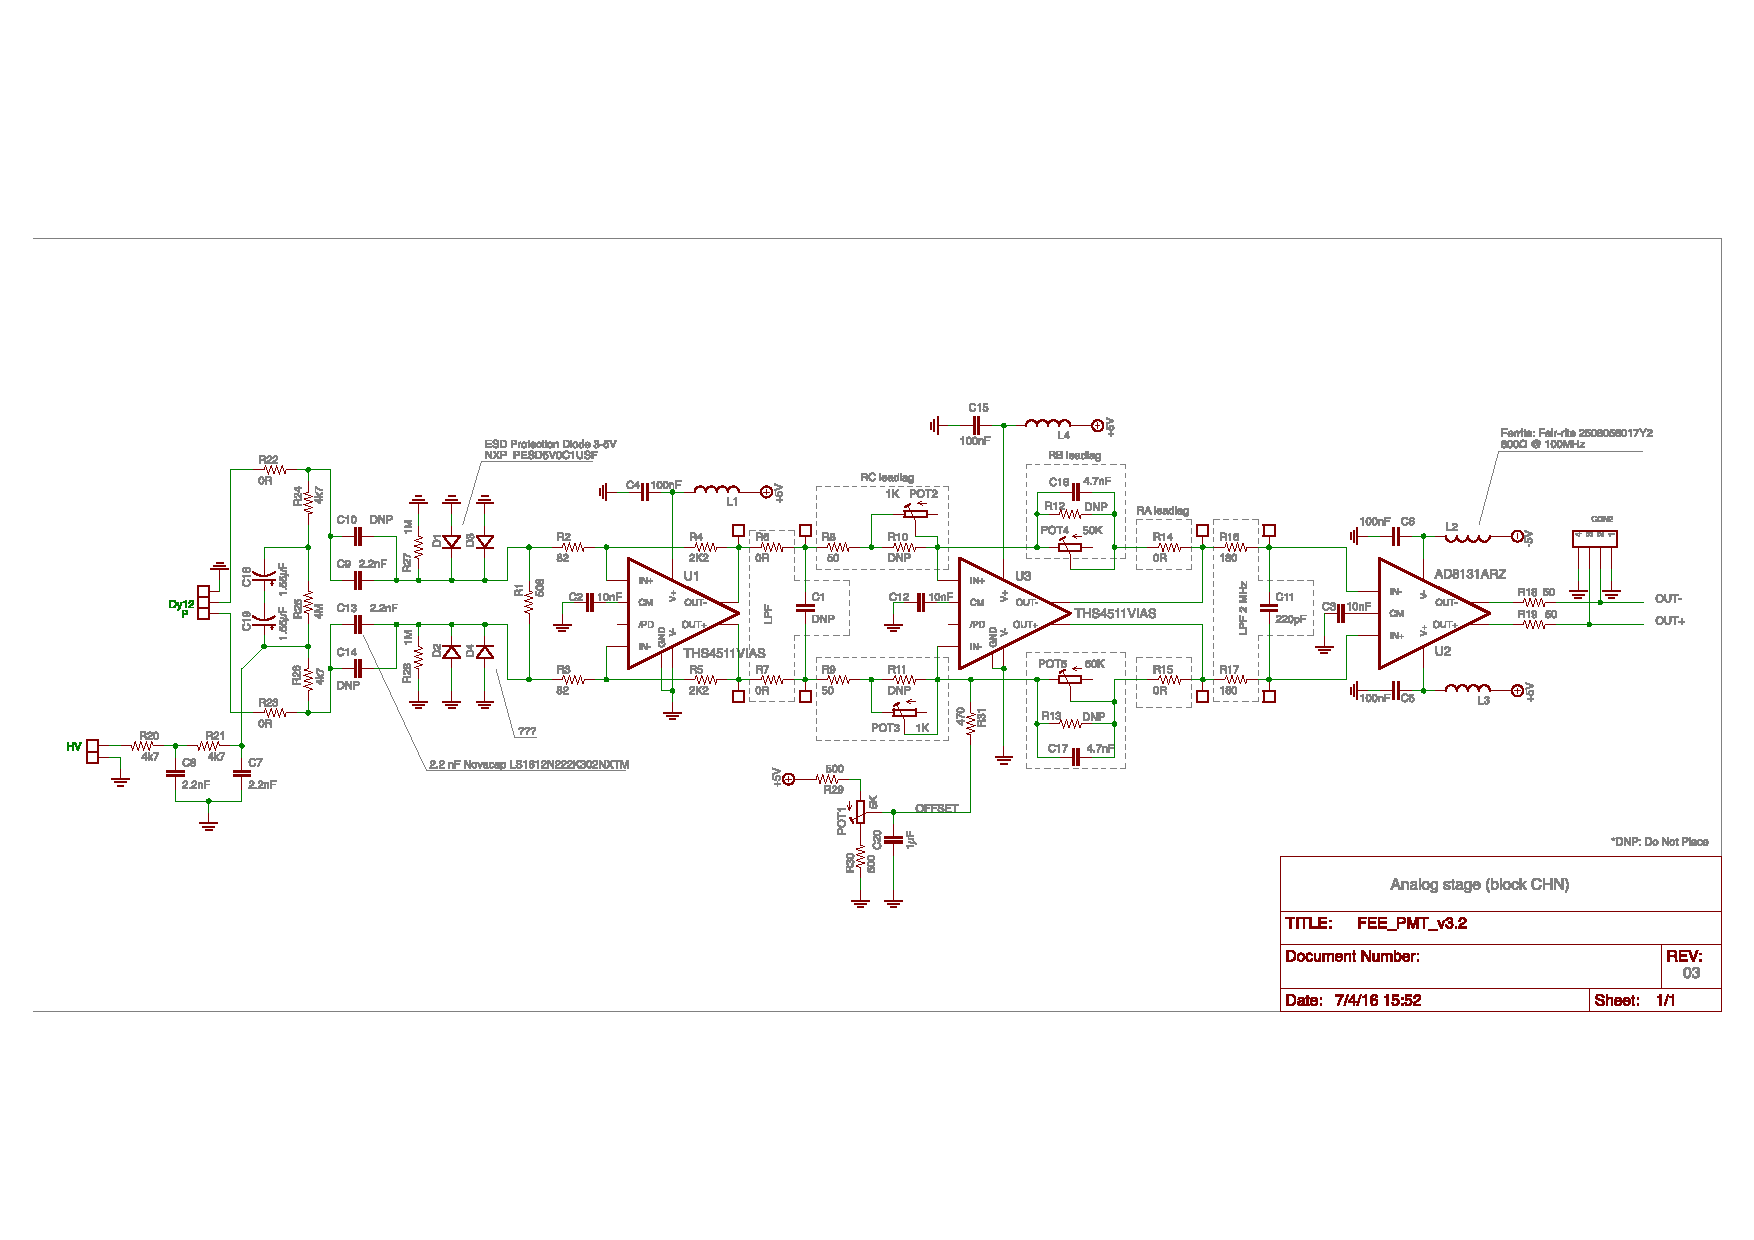
\includegraphics[height=4cm,width=0.95\textwidth]{img/FEE_PMT}
  \end{center}
  \caption{Schematics of the energy plane electronics. From top to bottom: Differential base (top), voltage regulators and four 2-channel hyerarchical blocks (middle) and one front-end channel circuit topology (bottom).  }
  \label{fig:fee_scheme} 
\end{figure}

There is more room for improvement by moving the first stage in the amplifier to the PMT base, as in this case larger resistors can be used and noise will be much lower. 
This is possible because there is no need to match impedances, as the amplifier would be very close to the base. The described approach will be explored in Spring 2016, in parallel to the tests
of the new front-end shown in figure \ref{fig:fee_scheme}.

\begin{figure}
  \begin{center}
    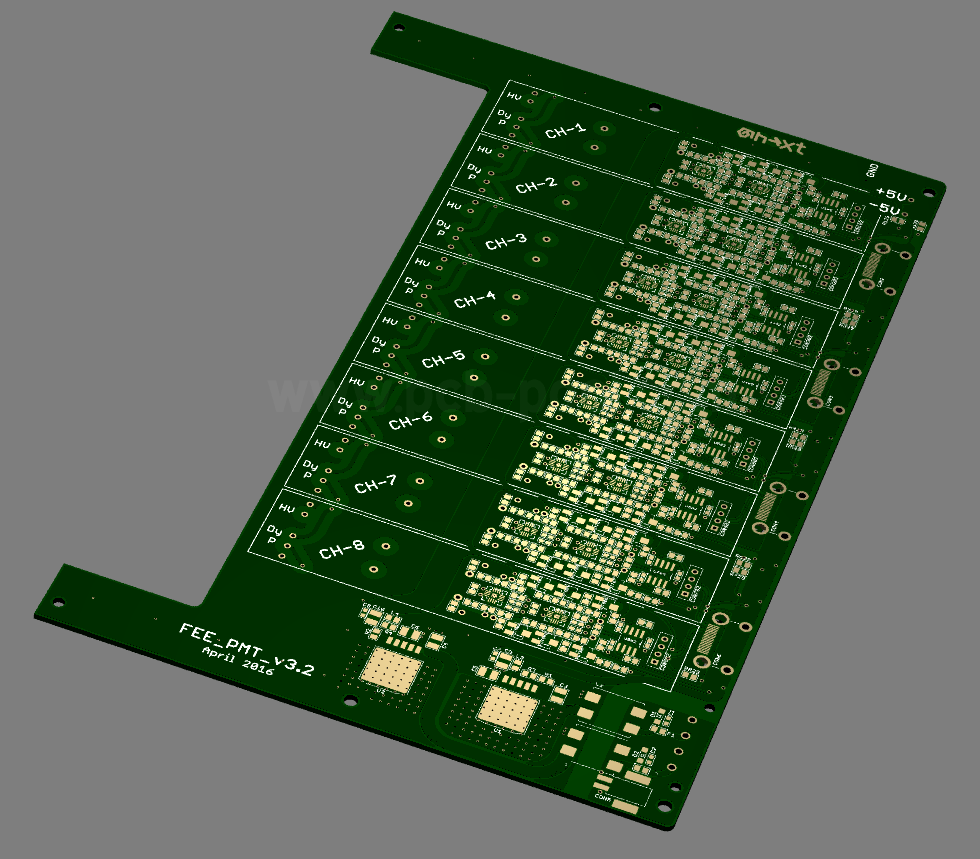
\includegraphics[height=8cm,width=0.95\textwidth]{img/FEE_PMT_PCB}
  \end{center}
  \caption{New PMT front-end PCB board, currently under production}
  \label{fig:fee_pcb_scheme} 
\end{figure}

\end{document}